\documentclass{article}
\usepackage{hyperref}
\hypersetup{
    colorlinks=true,
    linkcolor=blue,
    filecolor=magenta,      
    urlcolor=cyan,
    pdftitle={Overleaf Example},
    pdfpagemode=FullScreen,
    }
\usepackage[utf8]{inputenc}
\usepackage{geometry}
 \geometry{
 a4paper,
 total={170mm,257mm},
 left=20mm,
 top=20mm,
 }
 \usepackage{graphicx}
 \usepackage{titling}

 \title{Billiard table segmentation, balls location, segmentation and tracking
}
\author{Artico Giovanni Giacomin Marco Toffolon Mattia}
\date{July 2024}
 
\usepackage{fancyhdr}
\fancypagestyle{plain}{%  the preset of fancyhdr 
    \fancyhf{} % clear all header and footer fields
    \fancyfoot[L]{\thedate}
    \fancyhead[L]{Description of Assignment}
    \fancyhead[R]{\theauthor}
}
\makeatletter
\def\@maketitle{%
  \newpage
  \null
  \vskip 1em%
  \begin{center}%
  \let \footnote \thanks
    {\LARGE \@title \par}%
    \vskip 1em%
    %{\large \@date}%
  \end{center}%
  \par
  \vskip 1em}
\makeatother

\usepackage{lipsum}  

\begin{document}

\maketitle

\section*{Table segmentation (Artico Giovanni)}
The following assumptions were made for the segmentation of the table
\begin{itemize}
    \item the table is a uniform color and is a prevalent part of the image
    \item the table is centered (or close to being centered) in the image
\end{itemize}

It is going to be apparent the reason for these when the full algorithm for
the segmentation of the table is explained.
The first thing that was to be found was a rough segmentation of the table,
as finding the lines with only the Canny-transform of the full image would 
be problematic, as the strongest lines in the image are not only the table
fabric, but also the table itself and various other things in the image.
The initial approach was to use Otsu's thresholding, as the table is a uniform
color, therefore it is sensible to assume it would be thresholded the same
way throughout. This proved unfruitful, as the segmentation was too rough.
The second approach was to use kmeans clustering, in particular exploiting the
adaptability of the algorithm in order to use spatial features too to improve
the segmentation, as we assume the table is a continuous entity. Out of the k clusters obtained the most centered one was picked.
The segmentation obtained was fairly precise but contained multiple disconnected
components, however we can consider the table the biggest and pick it, in particular
before doing this operation open is applied in order to remove weakly connected objects.
the k (empirically) chosen was 3, as 2 lead to undersegmentation of the image and 4 to oversegmentation.
The resulting segmentation is precise in most cases, but given the nature of kmeans on some
images it fails, as it clusters some unrelated parts of the table with the fabric, due,
for example, to lighting.
For this reason further processing was required, given we have obtained a rough mask of
the table we now obtain the mean color of the image in the pixels where the mask is non-zero.
After this we use a color thresholding by distance from the mean and the same way we 
did before to obtain the largest connectedcomponent. In particular thresholding on the hue
is the most robust, in particular a low distance, 5, was chosen, but similar distances give similar
results.\par
after having obtained this result dilation is applied in order to remove some noise from the mask,
for example balls or other objects. Afterwards the hough transform is used to find the lines, 
with a threshold in order to remove similar lines.
The vertices of the table are found using the equations from \href{https://en.wikipedia.org/wiki/Line\%E2\%80\%93line\_intersection}{wikipedia}.
It is to note that the last frame is used for such frame as most of the time it doesn't contain the player in the table, being at the end of
a turn.

\begin{figure}
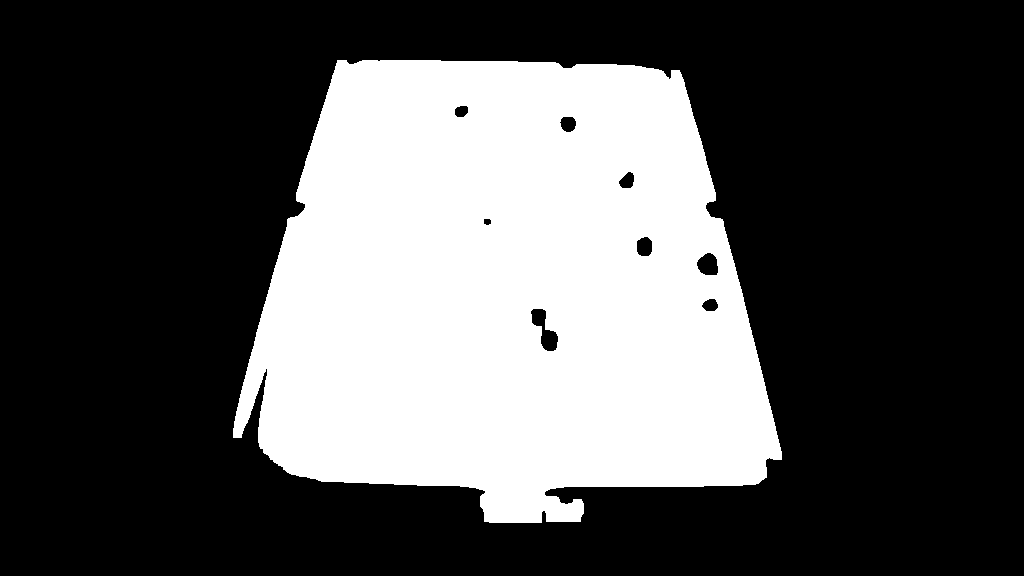
\includegraphics[width=0.6\textwidth]{./imgs/kmeans_cluster.png}
\caption{initial kmeans clustering result}
\end{figure}
\begin{figure}
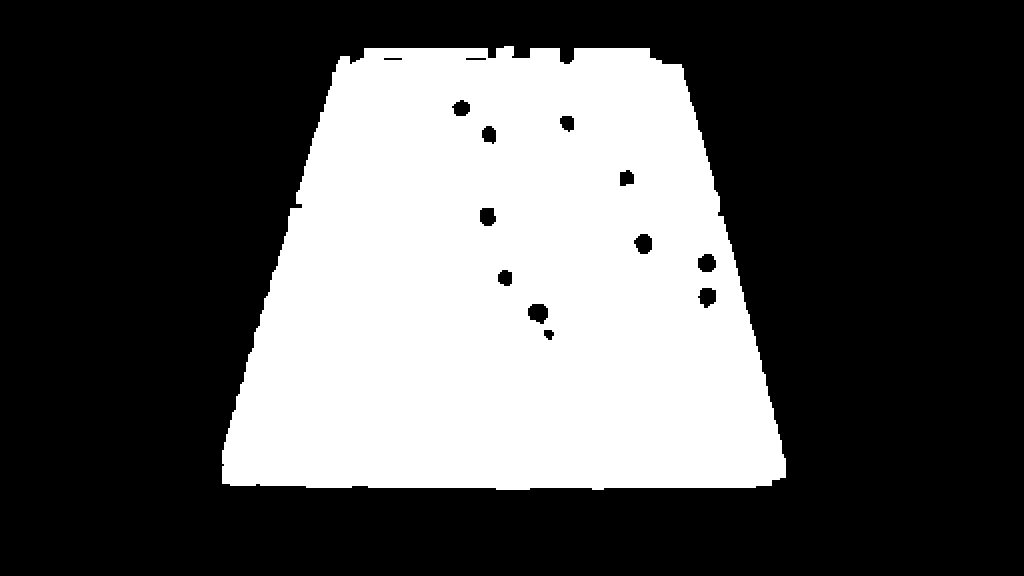
\includegraphics[width=0.6\textwidth]{./imgs/color_cluster.png}
\caption{final color clustering result}
\end{figure}

\section*{side recognition (Artico Giovanni)}
\section{Table Side Recognition}

The points are ordered from the upper-left-most point clockwise, but this doesn't give
any information on how the sides are ordered. It is unfortunately impossible (or out of my
mathematical capabilities) to find any meaningful geometrical relation between the sides
given the perspective deformations in some cases. The only feature we can go off of is the 
holes in the middle of the longer sides. The first operation was to obtain the rotated
rectangles containing the sides of the pool table, with a small width as to avoid 
keeping in the images unneeded information.\par 
Multiple approaches were tested to distinguish the two types of sides. The first was 
to use features (such as harris corners or SIFT), as intuitively they should appear 
on the holes and not on uniform sides as they should be classified as edges. This didn't
work, as the features and corners detected most of the time were spread throughout the 
considered sides most of the times as shown in \ref{fig:sift}.\par
The next approach was to try template matching between 3 different segments of the side image,
as the center contains a hole which should make the match significantly worse than
between the left and right segment. This does not work for two reasons:
\begin{itemize}
    \item because of the perspective the hole can appear in a part of the segment of the image that is not the center one
    \item because of the illumination and small imprecisions on the table segmentation the matching would fail even on the segments which should result similar
\end{itemize}
both of these are shown in figure \ref{fig:difficultside}.
\par
Ultimately the way to recognize the sides was the following:
\begin{enumerate}
    \item apply the Canny tranform on the initial image
    \item extract the rectangles from the image
    \item rotate the rectangles so that they are all horizontal
    \item apply sobel on the x-axis shown in image \ref{fig:sidestabol}
    \item sum over the contribution on the middle two quarters (as to avoid considering the corner holes) of the rectangles (normalized over the number of pixels contained in each)
    \item determine the longer sides by the highest contributions
\end{enumerate}
This works because of the nature of the edges on the sides: on shorter sides there
are mostly parallel lines, instead on longer there are strong edges orthogonal to the direction of the sides given by the holes.

\begin{figure}
    \centering
    \begin{subfigure}[b]{\textwidth}
    
\includegraphics[width=\textwidth]{./imgs/sobel_long_side.png}
    \caption{processed rectangle of a long side}\par
    \end{subfigure}\vspace{10pt}
    \begin{subfigure}[b]{\textwidth}
    
\includegraphics[width=\textwidth]{./imgs/sobel_short_side.png}
    \caption{processed rectangle of a long side}
    \end{subfigure}
    \caption{output of the processing of the sides}
    \label{fig:sidestabol}
\end{figure}
\begin{figure}
    \centering
    \begin{subfigure}[b]{\textwidth}
    
\includegraphics[width=\textwidth]{./imgs/bad_side_illumination_change.png}
    \caption{extreme illumination change in the  center of the side}\par
    \end{subfigure}\vspace{10pt}
    \begin{subfigure}[b]{\textwidth}
    
\includegraphics[length=\textwidth, angle=90]{./imgs/bad_side_warp.png}
    \caption{not centered hole}
    \end{subfigure}
    \caption{examples of difficulties in side recognition}
    \label{fig:difficultside}
\end{figure}
\begin{figure}
    \centering
    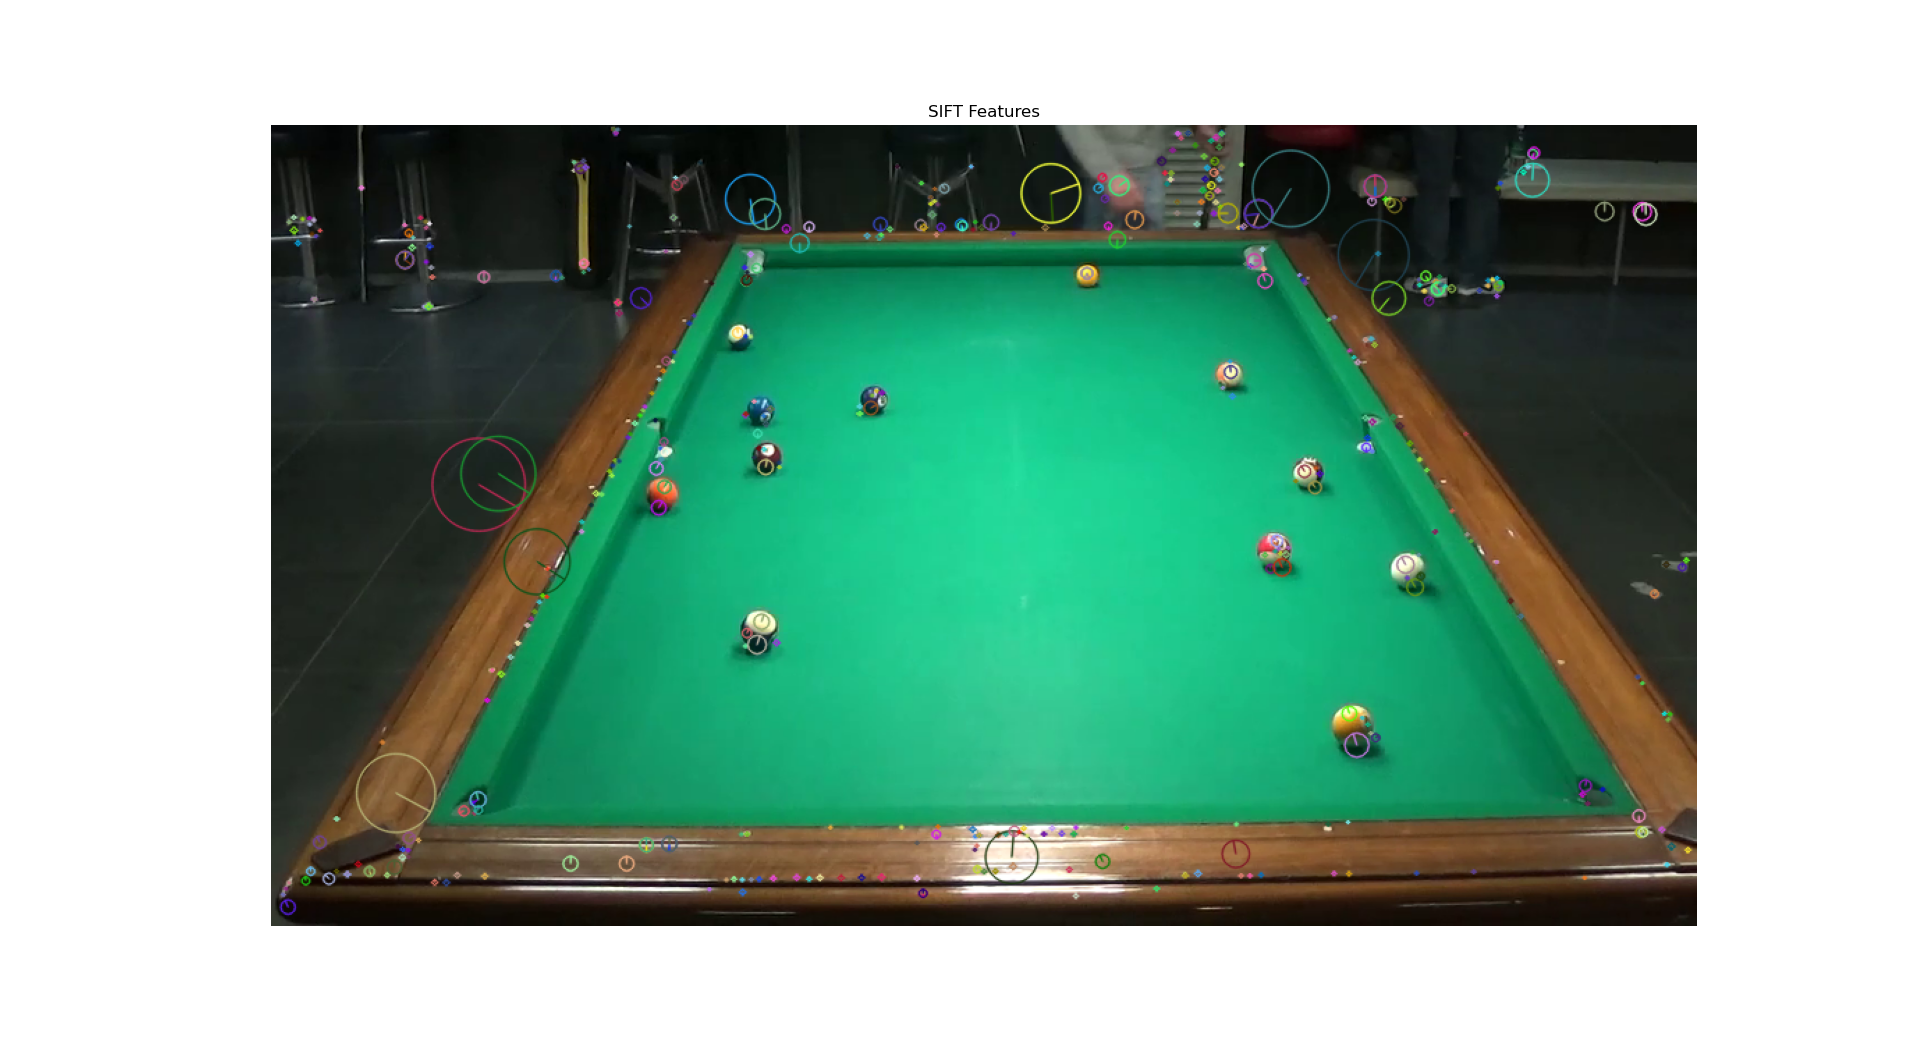
\includegraphics[width=0.5\textwidth]{./imgs/sift.png}
    \caption{Sift features in a sample image}
    \label{fig:sift}
\end{figure}

\end{document}
